\subsection{Model interpretability}
Considerable research efforts have been devoted to interpretable machine learning area with the pressing need to understand the behaviors of black box models. In other words, people would like to ascertain why a black box model makes such predictions. And the extent to explain the model behavior or its predictions in a human-understandable way is termed as interpretability \cite{kim2016examples}. In this thesis, we will use explainability or comprehensibility as its interchangeable term. 

Model explainability can be roughly categorized as two types: intrinsic interpretability and post-hoc interpretability \cite{molnar2019}. Intrinsic interpretability refers to models that are inherently interpretable, meaning that its predictions could be explained by model structures and model parameters. On the contrary to that, post-hoc interpretability is achieved by constructing a new model to provide explanations for the black box model. Particularly, post-hoc interpretability is mainly considered in the current context. Aside from the cognitive definition, it has to be noticed that there is no wide-spread mathematical formulae to define or measure the model interpretability. And the assumption that smaller models are more comprehensible than large models concerning the model size is problematic as pointed out by Freitas \cite{freitas2014comprehensible}. More specifically, we might argue that the model complexity is a determining factor to address the measurement of model interpretability. Nonetheless, how to assess the model complexity and how to link these two concepts are beyond our scope. 

Basically, models maintaining intrinsic interpretability are interpretable, which are known as interpretable models, including linear models or decision tree models. And it is not surprising that we can easily interpret model predictions through its parameters. For example, we train a logistic regression model to predict the house price. Evidently, we can decompose the house price prediction into the attributions of each feature, weighted by the coefficients. In this regard, an explanation for this prediction could be inferred from the feature impacts. In contrast, black box models are usually have low comprehensibility, with complex model structures and tremendous parameters. For instance, in the booming field of computer vision, practitioners prefer to apply deep neural networks to achieve sufficient performance with complex neural architectures, training procedures, regularization methods, and hyperparameters. Consequently, it is hardly possible for engineers to interpret the result.

Due to the fact the models with intrinsic interpretability are normally interpretable, we hence devote our efforts to the post-hoc interpretability on black box models. And it can be further classified as global interpretability and local interpretability \cite{du2018techniques}. Correspondingly, global interpretation methods and local interpretation methods are introduced as follows.

% In this chapter, previous works in areas that are related to the topic of this thesis will be covered. Firstly, we will introduce the model interpretation methods, which facilitate us to interpret predictions from black box models. Two groups of methods, including global interpretation methods and local interpretation methods, are explained respectively. And the last part will give an overview of subgroup discovery technique, focusing on the target concept and interestingness measure. 


\subsection{Model interpretation methods}

The main difference between global interpretability and local interpretability lies in the view of the dataset to be investigated, as displayed in Fig~\ref{fig:global_local}. The former highlights the impact of input variables based on the entire dataset, leading to an overall understanding of features. And the latter implies the justification for a specific decision, targeting at the instance level interpretation. There is a numerous number of papers that have imbued explainability in their methodology, and most techniques could be grouped into global interpretation methods and local interpretation methods, respectively. 

\begin{figure}[H]
	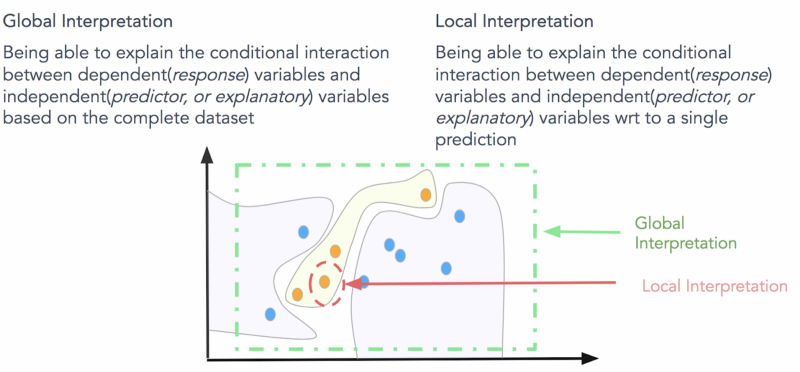
\includegraphics[width=0.9\textwidth]{imgs/global_local.png}
	\caption{Global interpretation view vs. Local interpretation view. Global interpretation explains the feature impact on a global view, based on the whole dataset. Local explanation focuses on the justification for a single instance by inspecting features.}
	\label{fig:global_local}
\end{figure}

\subsubsection{Global interpretation methods}

The global interpretation methods concentrate on the global view of the input variables, more specifically, they identify the most significant features that can largely affect model predictions of the entire dataset. Friedman proposed that the Partial Dependence Plot (PDP) was a global interpretation method which showed the marginal effect of a feature on the model predictions\cite{friedman2001greedy}. This method made clear the relationship between the selected feature and the predictions by adapting the values of the selected feature, and to characterize the feature impact on model predictions. Typically, some simple relationships such as linear or monotonic relation could be inferred from the plot directly. 

Another popular approach is called feature importance. There are many methods for assessment of feature importance. The default feature importance mechanism was proposed and implemented by the inventor of the RandomForest algorithm, which was to add up the Gini decreases for each variable over all trees in the forest and got the average. However, Strobl et al. had demonstrated that this method was biased and was not reliable in scenarios when the selected variable was biased in terms of the scale of measurement\cite{strobl2007bias}. Later, an improved strategy called permutation feature importance was described by Fisher et al. \cite{fisher2018model}. In his approach, the feature importance was estimated by the drop of prediction accuracy of the model after permuting the selected feature. A feature is regarded as "important" if prediction accuracy drops extensively after shuffling feature values as the model depends on the feature for the prediction. Conversely, a feature is "unimportant" if the accuracy is slightly dropped, which means the feature is hardly relied on for the model.

An alternative to permutation feature importance was SHAP feature importance, based on the magnitude of feature contribution using shapley values \cite{molnar2019}. To elucidate the idea, we could assume that the model prediction of an individual instance could be decomposed into feature attributions, and each attribution was estimated by the shapley value. Each feature had a corresponding shapley value for each instance. Thus, over the entire dataset, the SHAP feature importance was indicated by the mean absolute shapley values. 

% Permutation feature importance is based on the decrease in model performance. SHAP is based on magnitude of feature attributions.

\subsubsection{Local Interpretation methods}
%Influences do not provide any explanations about how the variable actually affects the response
Local interpretation methods aim at the instance level explanation which means each instance should be supplied with an explanation identifying the cause to the prediction. Following this idea, it leads us to the local surrogate methods, which are able to explain individual predictions of any black box models faithfully. As a concrete implementation of local surrogate models, Local interpretable model-agnostic explanations (LIME) was initially proposed by Ribeiro et al. \cite{ribeiro2016should}. The general idea was to train an interpretable model to approximate the predictions of the underlying black box model. Since the fitted model was interpretable, we hence could use this explanation model to give detailed explanations.

Another possible approach was to calculate the individual contribution of each feature in an instance to compose the final prediction as described in paper \cite{robnik2008explaining}. Inspired by this idea and the theoretical knowledge from the coalitional game theory, shapley value approach was highlighted to explain instance-level predictions with contributions of each feature values \cite{kononenko2010efficient}. Basically, each feature was assigned an importance score for a particular prediction, and the explanation could be derived from feature importance to some extent. 

However, by exploiting the shapley value approach, it was noticed that only a list of shapley values corresponding to each feature was generated to form an explanation for each model prediction, rather than an explanation model such as LIME, which failed to make judgments about the connections between input changes and prediction changes. To address those problems, Lundberg and Lee \cite{lundberg2017unified} proposed a unified framework for explaining predictions, which was based on the shapley value, and it was named SHAP(SHapley Additive exPlanations). In this unified framework, there was an novel approach called Kernel SHAP, which was the combination of linear LIME and shapley values. In this way, the intuitive connections between these two methods made this approach more promising. Besides, potential techniques to solve the computational performance problem in KernelSHAP was brought up as well. Tree SHAP, one of the variants in SHAP framework, was exhibited to deal with the computational complexity problem particularly for tree-based black box models. It implemented fast and efficient algorithms to calculate shapley values in comparison to Kernel SHAP. In addition, Deep SHAP was designed to improve computational efficiency when deep neural network was applied.


% This approach unified existing explanation methods and brought more clarity to the method space. They introduced the explanation model by treating the explanation of an individual prediction as a model.
\subsection{Review of subgroup discovery technique}

\subsubsection{Definition}
Recent developments of the research filed in knowledge discovery in databases have attracted much attention, where numerous methods are proposed to extract local patterns from large volumes of data  \cite{fayyad1996data}. Apart from the methods for mining local patterns such as discriminative patterns \cite{cheng2008direct} and emerging patterns \cite{dong1999efficient}, subgroup discovery (also called pattern mining) is established as a supervised and descriptive data mining technique. As defined in \cite{herrera2011overview}, in the subgroup discovery task, assuming we have a population of individuals and the corresponding property of interest, it aims to discover subgroups that are statistically "most interesting". To put it another way, the interesting subgroups have the most unusual distributional characteristics with respect to certain property of interest given by the target variable \cite{atzmueller2009fast}.

In a formal definition, the fundamental concepts of subgroup discovery task could be summarized by a quadruple (D, $\Sigma$, T, Q) \cite{lemmerich2014novel}. In the quadruple, D represents the dataset, which is formed by a group of instances. $\Sigma$ means the search space, consisting of a set of selection expressions, and the search space covers all the patterns that are going to be traversed through. Take an example, one of the selectors could look like: "sex=Male AND age>30". T implies the target concepts being exploited in the pattern mining task. Commonly, a single target concept, e.g. binary or numeric, is applied to the mining task. Nevertheless, multi-target concepts are also allowed given the existence of exceptional model mining framework \cite{leman2008exceptional}. Concerning the quality measure criteria, symbolized as Q, it is specified depending on the target concept.

\subsubsection{Quality measure}
To gain more insight, we present some quality measure criteria in this part. Since considerable research efforts have been devoted to study the binary target concept, the quality measure for binary target is well-investigated. One variant of the quality measure for binary target could be easily estimated by the parameters contained in a contingency table, which describes the distribution of positive/negative instances for the observed pattern and its complement subgroup, respectively. According to an investigation by Kloesgen et al. \cite{klosgen1996explora}, they proposed a prevalent family of quality measure, relating to the size of the subgroup and the difference between the target share in the subgroup and the target share in the general population. 

Correspondingly, several approaches to measure the quality of numeric attributes had been proposed, and a list of interestingness measures for numeric target concepts could be found in paper \cite{pieters2010subgroup}. Since a numeric attribute has certain characteristics, such as mean value or median value, therefore, the quality measure for a numeric target could be formalized by slightly adapting the quality function which is designed for binary targets. To be specific, chances were that the share of target in the subgroup and in the entire population could be replaced by the characteristic of the target. Generally, there were five categories of interestingness measure for numeric target, concluded by Lemmerich \cite{lemmerich2014novel}, which were mean-based measures, median-based measures, variance-based measures, distribution-based measures, and rank-based measures. 
Furthermore, as for a multi-target concept, the quality function had been described in a number of studies. And a general framework for multi-target quality functions was the exceptional model mining framework reported by Leman et al. \cite{leman2008exceptional}, proposing a variety of model classes, which contained the correlation model, the regression model, and the classification model class.   

\subsubsection{Subgroup discovery algorithms}
From previous part, four indispensable components were mentioned to define the problem of subgroup discovery. And in the following, algorithms to efficiently execute the subgroup discovery task is going to be considered. 

Unlike the choice of the quality measure which is mainly determined by a target concept in the subgroup discovery task, the mining algorithms are almost equivalent. And for a specific algorithm, three algorithmic components should be verified, which are enumeration strategy, data structure, and pruning strategy. Various enumeration strategies could be used, e.g. exhaustive methods, seeking to acquire the optimal subgroup by traversing through the whole search space. In contrast, heuristic approaches, normally a beam search strategy, was often used for subgroup discovery due to its efficiency, which aimed to find interesting patterns but not necessarily the optimal patterns in a short time \cite{clark1989cn2}. From data structure perspective, data was normally stored in a horizontal layout, e.g. tabular-formatted database. Instead, vertical data representations could also be used, which was covered in paper \cite{zaki2000scalable}. Besides, referring to the wide-spread FP-Growth algorithms, FP-tree structure was also applicable to data \cite{han2000mining}. Furthermore, considering the efficiency of algorithms, the pruning strategies was of critical importance. To determine the upper-quality bounds and safely prune parts of the search space, optimistic estimates could be explored as initially stated by Wrobel et al. \cite{wrobel1997algorithm}. In addition, to shrink the search space of subgroup discovery task, minimal support pruning strategy was useful by exploiting anti-monotone constraints.



